%%%%%%%%%%%%%%%%%%%%%%%%%%%%%%%%%%%%%%%%%%%%%%%%%%%%%%%%%%
\section{Evaluation}
\label{sec:evaluation}
%%%%%%%%%%%%%%%%%%%%%%%%%%%%%%%%%%%%%%%%%%%%%%%%%%%%%%%%%%
In practice, InvariMint not only infers useful summary models of the system
responsible for the input logs, but does so while addressing each of the
Synoptic limitations described in Section~\ref{sec:motivation}.

To evaluate the success of the formal languages approach, we also measure 
the relative efficiency of the two tools and compare
the final models generated by InvariMint with those generated by Synoptic.
% Discuss why walking the input traces didn't resolve the issue (Synoptic NFA to
% DFA translation)

%While implementing DFA
%minimization, for example, we realized an important distinction
%between invariants that are true for every trace (such as x Never Followed by y)
%and invariants that are only true globally (such as x Can be Followed by y).

%%%%%%%%%%%%%%%%%%%%%%%%%%%%%%%%%%%%%%%%%%%%%%%%%%%%%%%%%%
\subsection{Addressing Synoptic limitations}
%%%%%%%%%%%%%%%%%%%%%%%%%%%%%%%%%%%%%%%%%%%%%%%%%%%%%%%%%%

First, it is easy to add new types of invariants to InvariMint
as long as the invariants can be expressed as DFAs. This is how we recreated
Synoptic's initial model. This feature can also be used to more closely model
known features of systems. As one
example, consider some program in which an event $x$ must occur exactly twice before
some other event $y$. This would be a trivial addition to InvariMint, requiring
only some additional mining code and a regular expression for translating that
temporal relationship to a DFA. The same would be time
consuming to implement in Synoptic.

Second, InvariMint is much simpler to explain than Synoptic.
Whereas Synoptic uses highly specialized algorithms, DFA intersection and
minimization are both common, widely understood techniques for manipulating
state machines.

Third, InvariMint deterministically generates a globally minimal model that
satisfies all mined invariants. In contrast to Synoptic's refinement phase, the
order in which InvariMint intersects invariants has no affect on the final
model.

Finally, by referencing the input logs only once to mine invariants rather than continually
while constructing the final model, InvariMint scales better than
Synoptic on large logs.

%%%%%%%%%%%%%%%%%%%%%%%%%%%%%%%%%%%%%%%%%%%%%%%%%%%%%%%%%%
\subsection{Performance}
%%%%%%%%%%%%%%%%%%%%%%%%%%%%%%%%%%%%%%%%%%%%%%%%%%%%%%%%%%
InvariMint offers better scalability than Synoptic with respect to the size of
the input log because the algorithm avoids repeated references to the log while
inferring the final model. We measured scalability with respect to the size
of the input log by timing both Synoptic and InvariMint on logs of varying
size from the Reverse Traceroute system~\cite{ReverseTraceroute} which
determines return paths for packets on the Internet.
Figure~\ref{fig:performanceLogLine} plots the run time in milliseconds of both Synoptic and
InvariMint
on input logs ranging from 250 to 64,000 lines. 
Recorded times are the average of 10 executions measured after 10 warm-up
runs. 

As the size of the log increases, InvariMint is far more
efficient than Synoptic. Eventually parsing the input log and mining invariants dominates InvariMint's run
time as opposed
to the time taken to infer the final model.

These experiments only confirm that InvariMint is efficient with respect to the
size of the input log. In the future we hope to measure InvariMint's scalability
with respect to the number of log invariants. For all of the Reverse Traceroute logs,
the number of invariants (both mined and implicit) is lower than 200.

\begin{figure}
  \center
  {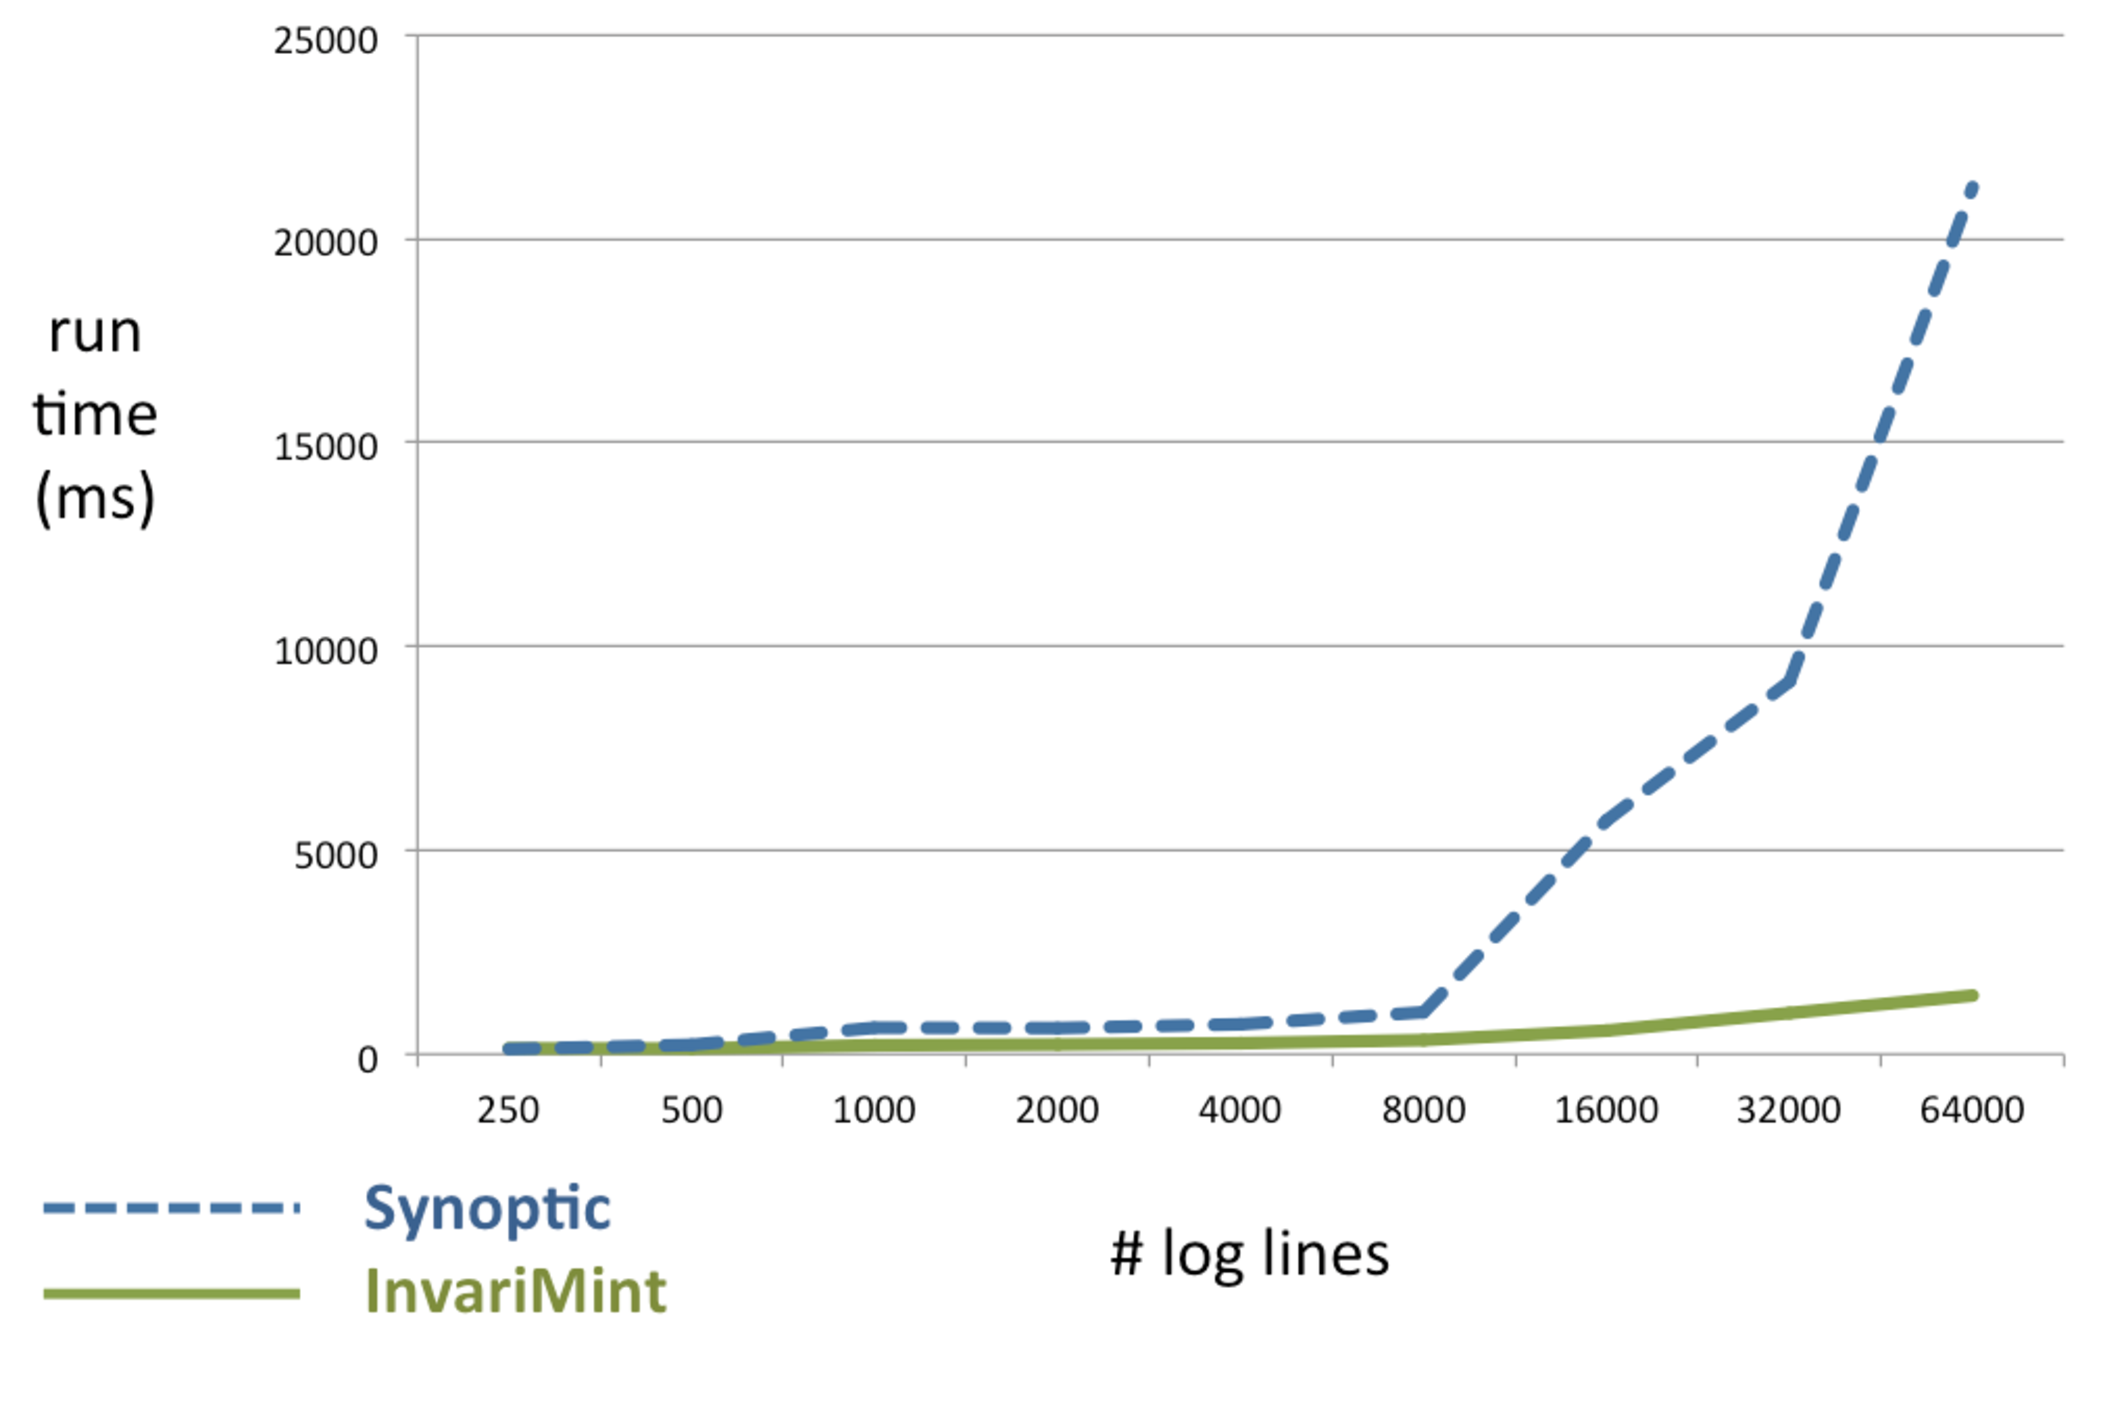
\includegraphics[width=\columnwidth]{fig/performanceLogLines.pdf}}
  \caption{Run time of Synoptic versus InvariMint as the size of the input log
  increased.}
  \label{fig:performanceLogLine}
\end{figure}

%%%%%%%%%%%%%%%%%%%%%%%%%%%%%%%%%%%%%%%%%%%%%%%%%%%%%%%%%%
\subsection{Model comparisons}
%%%%%%%%%%%%%%%%%%%%%%%%%%%%%%%%%%%%%%%%%%%%%%%%%%%%%%%%%%
Despite satisfying the same invariants and accepting all of the input traces,
InvariMint and Synoptic do not generate identical models. Exploring these
differences is useful for thinking about discrepancies between the techniques
and is important because the differences may make it harder or easier for
developers to use the models.

\begin{figure*}[t]
  \center
  {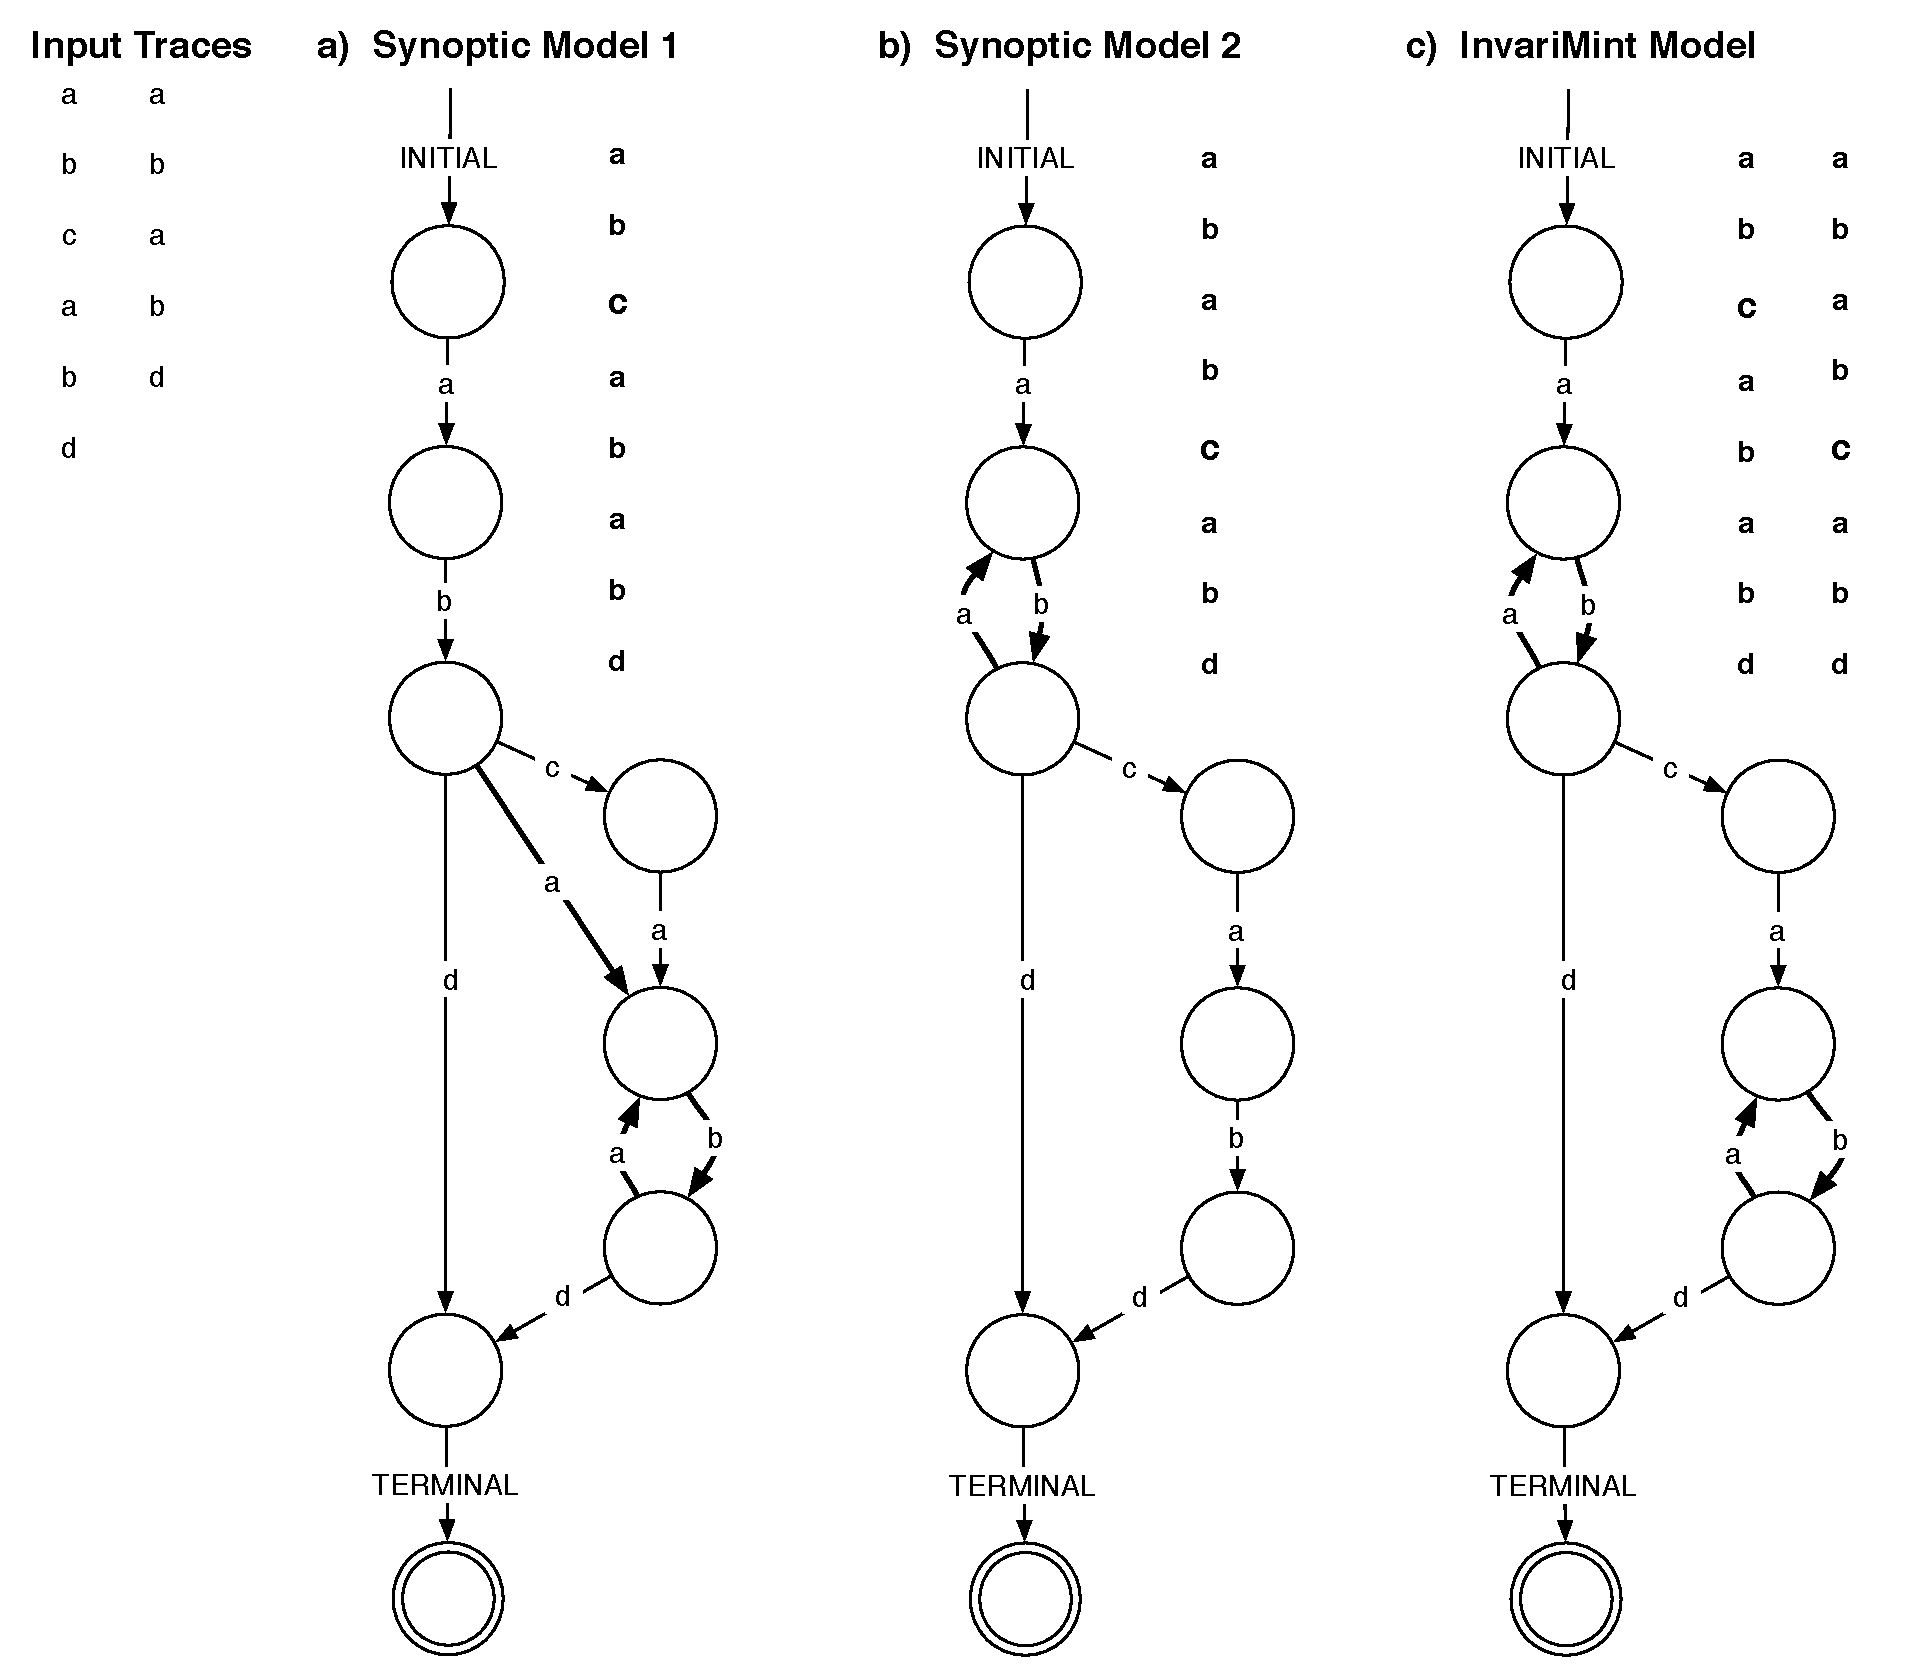
\includegraphics[width=\linewidth]{fig/union.pdf}}
  \caption{Models a and b are possible final Synoptic models given the provided input
  traces. Next to each model is an example of a synthetic trace accepted by that
  model but not the other. The corresponding InvariMint model, c, accepts the union
  of synthetic traces accepted by both Synoptic models.} 
  \label{fig:synthetic}
\end{figure*}

%%%%%%%%%%%%%%%%%%%%%%%%%%%%%%%%%%%%%%%%%%%%%%%%%%%%%%%%%%
\subsubsection{Union of Synoptic models}
%%%%%%%%%%%%%%%%%%%%%%%%%%%%%%%%%%%%%%%%%%%%%%%%%%%%%%%%%%
Synoptic generates a final model that accepts all of the input traces as well as
some synthetic traces satisfying all of the mined and immediate invariants.
Because Synoptic is non-deterministic, the set of synthetic traces accepted by
the final model may vary depending on the order in which invariants were
satisfied during refinement. Figure~\ref{fig:synthetic} illustrates an example
of this: there are two possible final Synoptic models satisfying
all log invariants for the given input traces, and these models accept a different set of synthetic traces.

This can be problematic for users. Consider the developer who finds a bug in
their system by examining a Synoptic model. After modifying their system, the
developer provides new input logs to Synoptic to verify that the bug is fixed.
Though the buggy behavior is gone, it is possible that some unrelated part of
the model has changed, leaving the developer to wonder whether they
unintentionally introduced additional modifications to the system.

InvariMint solves this issue by generating models deterministically.
Though not formally verified, we hypothesize that the final InvariMint model 
accepts the union of all possible synthetic traces accepted by any of
the corresponding Synoptic models. This is the case for the InvariMint
model in 
Figure~\ref{fig:synthetic} which accepts both sets of synthetic traces generated by different
Synoptic models.


Figure~\ref{fig:language-venn}
provides a visual illustration for the intuition behind this idea: the language accepted by InvariMint
is precisely the intersection of the initial model and each of the mined
invariants. Synoptic accepts a language that is some subset of that
intersection.

The union property is poised to have a number of benefits. First, it provides a bound for the set of
possible final Synoptic models which was previously an ambiguous space. Second,
the additional synthetic traces may be useful for users attempting
to predict the range of possible system behaviors for purposes such as generating
additional test cases. In future work we hope to conduct a
usability study to evaluate the utility of additional
synthetic traces. 

%%%%%%%%%%%%%%%%%%%%%%%%%%%%%%%%%%%%%%%%%%%%%%%%%%%%%%%%%%
\subsubsection{Spurious Edges}
%%%%%%%%%%%%%%%%%%%%%%%%%%%%%%%%%%%%%%%%%%%%%%%%%%%%%%%%%%
Assuming that the languages accepted by Synoptic models are always a subset of
the language accepted by a corresponding InvariMint model, the next question
is whether 
there are any traces accepted by an InvariMint model that are not
accepted by \emph{any} corresponding Synoptic model.

In fact, InvariMint models can accept synthetic traces that do not exist in any
corresponding Synoptic model. These are caused by \textbf{spurious edges} and
highlight an important distinction between the two techniques: underlying the Synoptic models
are specific event instances, whereas
InvariMint deals only with event types.

During refinement and coarsening, 
Synoptic maintains partitions containing one or more
concrete instances of that partition's event type from some input trace.
For each event instance $a$ in the partition, there exists an incoming edge from some
partition containing the event instance that immediately preceded that instance $a$ and there
exists an outgoing edge that leads to some partition containing
the event instance that immediately followed $a$.
Synoptic models thus have the property that every edge in the final model corresponds
to two successive events in at least one input trace. In other words, every edge
respects the \emph{edge-coverage property}.

The Synoptic model accepts some synthetic traces -- traces not contained within
the set of 
input traces -- but these are limited by the edge-coverage property.

InvariMint models in contrast have no notion of input traces and are concerned
only with the temporal relationships between event types.
Because InvariMint models
do not have the edge-coverage property, they are
more permissive than Synoptic models, accepting a wider range of synthetic
traces.

Figure~\ref{fig:spurious} illustrates an example of this.
The Synoptic model allows only the set of input traces in its final model.
The InvariMint model allows 
an additional $INITIAL-x-a-y-TERMINAL$ synthetic trace because no mined
invariant prohibit it.

\begin{figure}[t!]
   \center
   {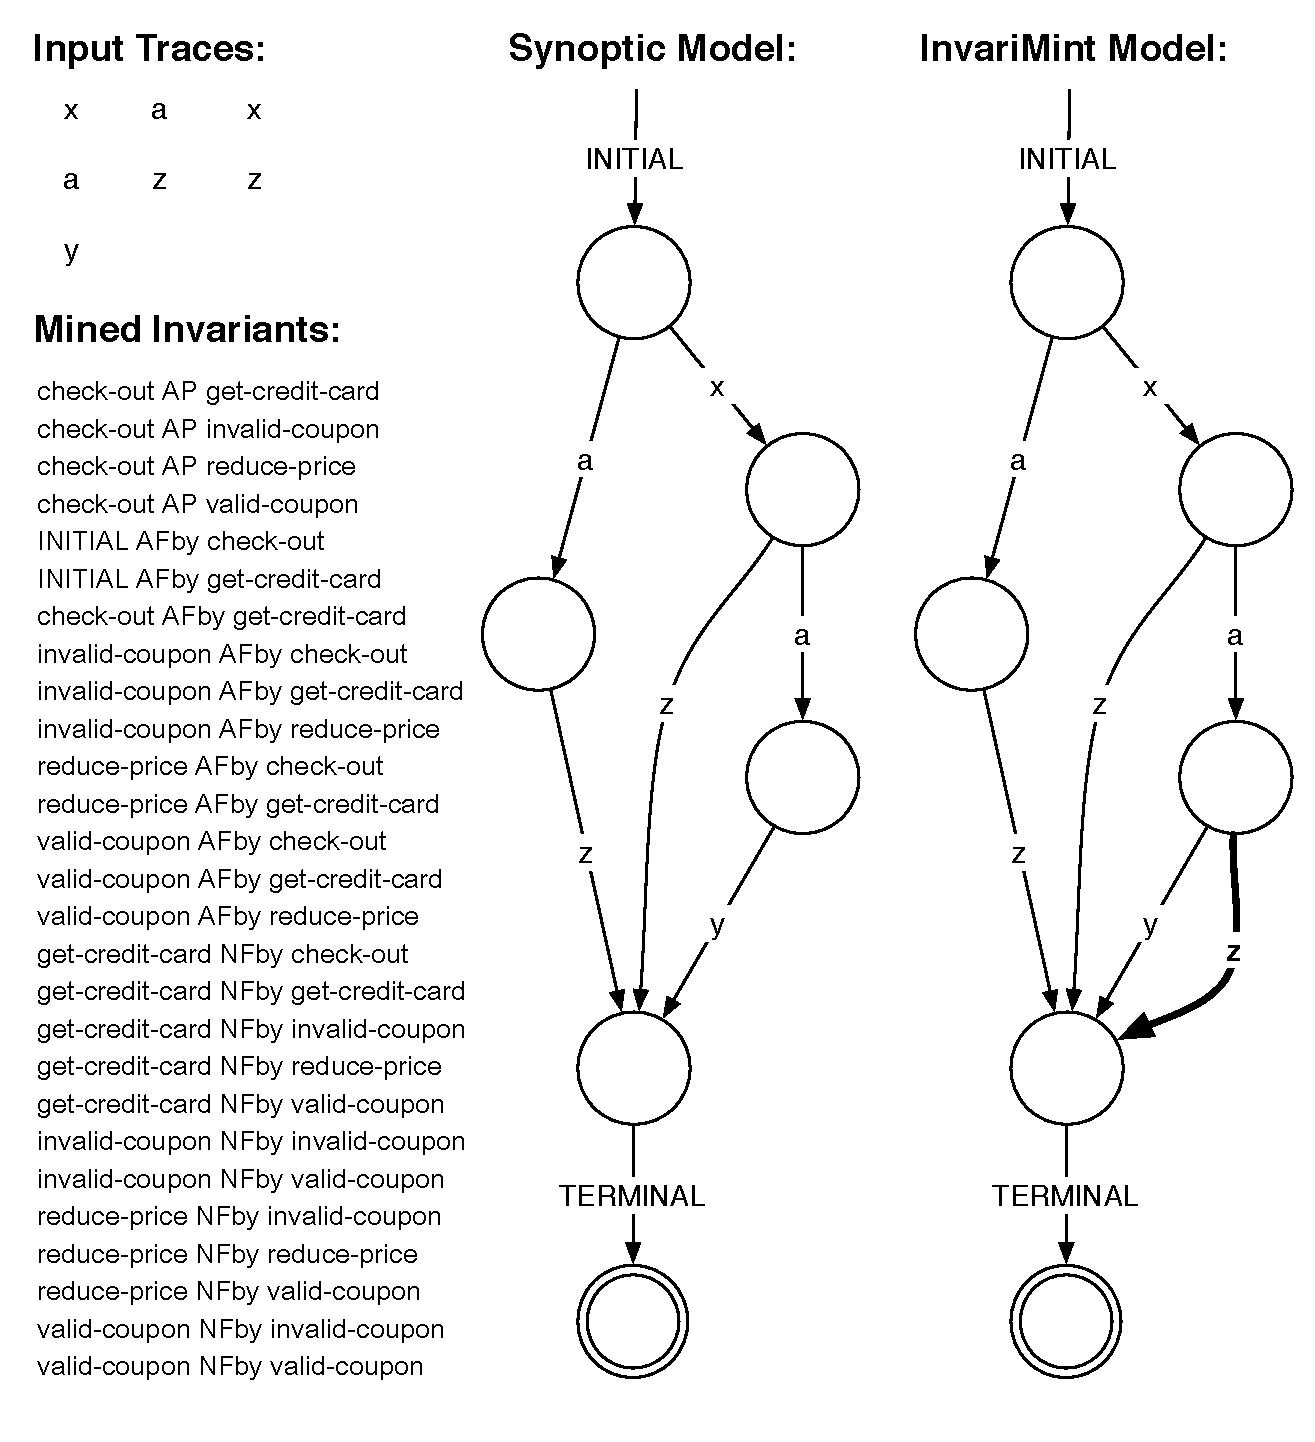
\includegraphics[width=0.95\columnwidth]{fig/spurious.pdf}}
   \smallskip
   \caption{An abstract example of a spurious edge in an InvariMint model. The input traces
   and mined invariants are shown at left. Each edge in the Synoptic model
   (translated to an InvariMint-style DFA for easier comparison)
   corresponds directly to an event in some input trace. The InvariMint
   model is almost identical to the Synoptic model but includes an additional 
   $z$ edge from $a$ to $TERMINAL$. This transition does not map to any event in the
   input logs so violates the edge-coverage property and is spurious.
   This spurious $z$ edge is allowed by InvariMint because elsewhere an event
   $z$
   immediately followed an event $a$ and none of the other invariants restrict this
   particular instance of $z$.}
   \label{fig:spurious}
\end{figure}

More concretely, because an event $z$ immediately followed an event
$a$ in at least one input trace, the $a~NIFby~z$ invariant was not mined during
construction of 
the initial model and every instance of an event $a$ in the InvariMint model can be
immediately followed by an event $z$ unless prohibited by 
some other invariant. The left-most event $a$ in the InvariMint model in Figure~\ref{fig:spurious},
for example, is not followed by an event $y$ even though $y$ can immediately
follow $a$ because that would allow traces violating the 
$x~AP~y$ invariant.

The $z$ edge in the InvariMint synthetic trace would map to an $a$--$z$
edge in the corresponding state-based model used by Synoptic. There does not
exist any input trace that would traverse the $z$ edge in this model, and thus
the edge is an 
example of a spurious edge.

%%%%%%%%%%%%%%%%%%%%%%%%%%%%%%%%%%%%%%%
\subsubsection{Removing spurious edges}
%%%%%%%%%%%%%%%%%%%%%%%%%%%%%%%%%%%%%%%
To best approximate Synoptic, InvariMint models should not contain any spurious
edges. However, we have not yet developed an adequate way to remove these 
edges from InvariMint models.

One plausible way to remove spurious edges is to traverse the input traces
during one additional post-processing step and remove any edges in the final
InvariMint model violating the edge-coverage property.

A problem with this
strategy is that Synoptic generates NFAs with the edge-coverage property whereas
InvariMint generates DFAs. Translating Synoptic models to DFAs generates models
that accept the same language as the original model but creates a model that may
violate the edge-coverage
property.

This is due to additional edges and states introduced by the NFA-to-DFA
translation. Thus InvariMint models can contain
edges
that both violate the edge-coverage property and are spurious, but 
can also contain edges that 
violate the edge coverage property but if removed would restrict
the language of the model in ways that the corresponding Synoptic model does not.

For example, applying the post-processing operation to remove spurious edges
on the InvariMint model in Figure~\ref{fig:synthetic} would remove the edges
that allow the a-b-c-a-b-a-b-d synthetic trace. The resulting language 
would no longer be the union of languages accepted by all Synoptic models.

Spurious edges reveal a loss of context in InvariMint models. Synoptic models
are more nuanced, preserving greater trace-specific information.
Given a Synoptic model, it is possible to query specific edges
to reveal precisely which 
input traces allowed that transition between events. This can be useful, for
example, to pinpoint
the precise executions in which a bug appeared. The mined invariants used by
InvariMint do not capture any trace specific information.

Less context-sensitivity is not necessarily a bad thing: the InvariMint models
are more
general and ignore individual trace idiosyncrasies, leading to smaller
models as more states can be merged. As the scale of the input grows, 
model brevity and efficiency may prove to be more valuable than trace-specific
information.
